\documentclass[a4paper,oneside,final,12pt,russian]{article}
\usepackage{cmap}
\usepackage[utf8]{inputenc}
\usepackage[T2A,T1]{fontenc}
\usepackage[russian]{babel}
\newcommand{\comment}[1]{}
\usepackage{graphicx}
\usepackage{caption}
%\usepackage{float}
\usepackage{subcaption}
\usepackage{amsthm}
\usepackage{wrapfig}
\usepackage{svg}
\usepackage{listings}
\usepackage{xcolor}
%\usepackage{apacite}
\usepackage[pdftex,hidelinks,bookmarks=true]{hyperref}
\usepackage{etoolbox}
\usepackage{natbib}
\usepackage{url}
\newcounter{bibcount}
\usepackage[nottoc]{tocbibind}
\newtheorem{theorem}{Лемма}
\graphicspath{ {images/} }

\definecolor{codegreen}{rgb}{0,0.6,0}
\definecolor{codegray}{rgb}{0.5,0.5,0.5}
\definecolor{codepurple}{rgb}{0.58,0,0.82}
\definecolor{backcolour}{rgb}{0.95,0.95,0.92}

\lstdefinestyle{mystyle}{
backgroundcolor=\color{backcolour},
commentstyle=\color{codegreen},
keywordstyle=\color{magenta},
numberstyle=\tiny\color{codegray},
stringstyle=\color{codepurple},
basicstyle=\ttfamily\footnotesize,
breakatwhitespace=false,
breaklines=true,
captionpos=b,
keepspaces=true,
numbers=left,
numbersep=5pt,
showspaces=false,
showstringspaces=false,
showtabs=false,
tabsize=2
}

\lstset{style=mystyle}

\begin{document}
    \newpage
    \begin{center}
    Федеральное государственное автономное образовательное учреждение\\
    высшего образования\\
    <<Московский физико-технический институт (национальный исследовательский университет)>>\\
    Физтех-школа радиотехники и компьютерных технологий\\
    Кафедра теоретической и прикладной информатики\\
\end{center}

\vspace{2mm}

\begin{flushleft}
    \textbf{Направление подготовки:} 03.03.01 Прикладные математика и физика\\
    \textbf{Направленность (профиль) подготовки:} Радиотехника и компьютерные технологии\\
\end{flushleft}

\vspace{24mm}

\begin{center}%Применение сжатых индексов для полнотекстового поиска
    \large{\textbf{ПРИМЕНЕНИЕ СЖАТЫХ ИНДЕКСОВ\\ДЛЯ ПОЛНОТЕКСТОВОГО ПОИСКА}}\\
    (бакалаврская работа)\\
\end{center}

\vspace{20mm}

\hspace{90mm}
\begin{minipage}{0.4\textwidth}
    \begin{flushleft}
        \textbf{Студент:}\\Соколов Вадим Андреевич\\
        \vspace{4mm}
        \hrulefill\\
        {\centering\scriptsize\textit{(подпись студента)}\\}
        \textbf{Научный руководитель:}\\Неганов Алексей Михайлович\\
        \vspace{4mm}
        \hrulefill\\
        {\centering\scriptsize\textit{(подпись научного руководителя)}\\}
    \end{flushleft}
\end{minipage}

\vspace*{\fill}

\begin{center}
    Москва 2021
\end{center}

\thispagestyle{empty}
    \newpage
\section*{Аннотация}

\textbf{Цели и задачи работы.}

Данная работа посвящена исследованию структур данных,
использующих сжатые индексы (succinct index) для хранения текстовой информации.

Целью данной работы является проверка эффективности различных методов сжатия данных.
Исследуется применимость сжатых индексов на практике при работе с данными определенного типа.
Производится сравнение как с традиционными решениями (suffix array), так и с более современными (radix tree),
использующими подход для индексирования, отличный от исследуемых структур данных.


\textbf{Полученные результаты.}


Удалось получить сравнительные характеристики работы традиционных структур данных.
Были измерены и проанализированы:
\begin{enumerate}
    \item объем потребляемой памяти;
    \item время, требуемое для вставки / поиска подстроки;
\end{enumerate}

На языке Go реализована сжатая структура данных succinct suffix array. Приведены результаты потребления памяти
для хранения сжатого индекса и скорости поиска подстроки в тесте.



    \newpage
\tableofcontents
\newpage

\section{Введение}

% inverted index
% bioinformatics is important
% pattern matching is used in it
% so it is crusial to work with substrings

Работа с текстовыми данными находит применение в широком спектре задач современной компьютерной индустрии.
При работе с текстовыми данными очень часто используется inverted index \cite{zobel2006inverted}. Эта структура данных
позволяет индексировать слова в документах. Но существует ряд проблем, для которых индексирование слов
не является решением.
Например, в ряде задач биоинформатики \cite{tsuruoka2008facta} присутствует поиск паттерна в ДНК-коде или коде белковой структуры,
которые не представляют собой слова и соответственно inverted index для них не применим.
Аналогично в некоторых восточных языках (китайский, арабский) текст не делится на отдельные слова.
Дополнительно, inverted index ограничен при поиске строки, похожей на искомую, но не совпадающую с ней в точности.
Например, при поиске информации в поисковых системах, где в качестве запроса используется текст, содержащий
орфографические ошибки или другие неточности, inverted index не сможет дать пользователю искомый ответ.
В этих случаях используются индексы, построенные на отсортированных суффиксах исходного текста.
Примером такого индекса является суффиксный массив (suffix array) \cite{manber1993suffix}. В нем реализована возможность поиска подстроки,
что позволяет решать задачи, недоступные для inverted index. В свою очередь, suffix array может занимать
место, превосходящее исходный текст до 50 раз.

Рост количества информации в Интернете приводит к дополнительным издержкам при хранении и поиске данных.
В связи с этим существует необходимость исследования различных способов уменьшения потребляемой памяти без
существенных затрат на поиск данных.

Одним из возможных решений такого рода задач является применение сжатых структур данных
(succinct data structures) \cite{jacobson1988succinct}.
В зависимости от степени сжатия информации структуры данных различаются на имплицитные, сжатые и компактные.
Сжатые структуры используют близкое к теоретически минимальному количеству информации для хранения данных.
Кроме того, в отличие от архивов и других сжатых представлений, остается возможность
эффективно выполнять операции поиска.
Предположим, что для хранения некоторого количества данных требуется Z бит.
Сжатые структуры данных занимают \(Z + o(Z)\) бит. Например структура данных, занимающая \(Z + \ln(Z)\) бит памяти,
является сжатой.


Данные не всегда сжимаемы. Кроме того, не любые данные целесообразно сжимать с точки зрения эффективности
их использования в несжатом виде. В этой работе предлагается рассмотреть сжатие индекса суффиксного массива,
построенного для различных тектовых данных. При этом сам текст остается в несжатом виде.


Для того чтобы представить данные в сжатом виде, необходимо подготовить их
в специальном промежуточном формате. В этой работе используется алгоритм Элиас-Фано \cite{pibiri2014dynamic},
позволяющий сжимать возрастающие последовательности неотрицательных целых чисел.
Исследование направлено на изучение потребления памяти для сжатого представления суффиксного массива.
Реализованы функции поиска подстроки, и произведен анализ их эффективности.



\newpage
\section{Постановка задачи}
\newpage



\newpage
\section{Обзор литературы}
%1. Common problems and common technologies [+]
% - Text search +
% - Self Index +
% - Problems with self indexation +
% - Full text search with substrings +
%2. SA: overview, complexity, usage         [+]
%3. Radix: overview, complexity, usage      [+]
%4. Succinct data                           [+]
%5. CSA                                     [+]
%6. PSI                                     [+]
%7. Regenerating SA from PSI                [+]
%8. EF                                      [+]
%9. My CSA                                  []
%10.Complexity                              []

\textbf{Поиск по тексту}

В настоящее время Интернет каждый день пополняется большим количеством данных.
Поэтому чрезвычайно важно организовать поиск нужной информации \emph{эффективно}.
При поиске по документам применяется индексирование.
Традиционным для индексирования текста является \emph{inverted index}.
Это структура данных, в которой для каждого слова коллекции документов в соответствующем списке
перечислены все документы в коллекции, в которых оно встретилось.
При обработке многословного запроса берётся пересечение списков, соответствующих каждому из слов запроса.

\textbf{Проблемы традиционных подходов}

На практике встречаются случаи, в которых невозможно использовать традиционный поиск по словам.
Модель поиска, в которой задачей является найти орфографически близкие слова (\emph{fuzzy search}),
использующаяся для корректирования правописания во многих текстовых редакторах,
не позволяет решать проблему при помощи поиска по словам.
То же самое касается других систем, в которых используется \emph{pattern matching}.
Еще одним примером текстов, в которых сложно применять традиционный поиск,
являются некоторые восточные языки.
В них слова не делятся пробелами между собой, что делает трудным использование \emph{inverted index}.
Наконец, к <<неудобным>> можно отнести длинные тексты, составленные из алфавита с малым набором символов.
Характерными примерами таких текстов являются ДНК и код белковой структуры.
Этот текст не делится на слова, что является ключевой проблемой при использовании \emph{inverted index}.

Для решения таких проблем необходимо использовать поиск по подстрокам.
Существующие подходы (prefix tree, suffix array) занимают много места, поэтому не являются эффективными.
Например, для prefix tree, хранящем в себе n слов со средним количеством символов в каждом слове $C$,
требуется $O(n \cdot C)$ памяти.
Рассмотрим подробнее suffix array, как один из самых востребованных способов индексации текстовой информации.

\textbf{Полнотекстовый поиск при помощи suffix array}

Suffix array -- это структура данных, используемая в полнотекстовой индексации, позволяющая выполнять
поиск подстроки в тексте размером n символов за $O(\log{}n)$.
При этом для хранения n слов в suffix array необходимо $O(n \log{}n)$ памяти.
Так для ASCII-текста размером $2^{32}$ требуется $2^{32} \cdot 8 = 32$ гигабит пространства памяти.
Для такого текста suffix array должен содержать элементы размером 32 бита.
Тогда размер suffix array достигает $2^{32} \cdot 32 = 128$ гигабит пространства памяти,
что в 4 раза превышает размер исходного текста.

Suffix array представляет собой отсортированную в лексикографическом порядке
последовательность суффиксов. Для лучшего понимания устройства suffix array, рассмотрим эту структуру данных на примере индексирования
слова mississippi:
\\(0) mississippi
\\(1) ississippi
\\(2) ssissippi
\\(3) sissippi
\\(4) issippi
\\(5) ssippi
\\(6) sippi
\\(7) ippi
\\(8) ppi
\\(9) pi
\\(10) i

Suffix array, составленный из таких суффиксов, будет иметь вид:

10 7 4 1 0 9 8 6 3 5 2

Обычно конец документа обозначается специальным символом, не входящим в алфавит хранящегося в массиве текста.
В качестве такого разделителя в этой работе был выбран символ доллара \$.
Современные подходы по построению suffix array позволяют конструировать структуру данных за $O(n)$.

\textbf{Radix tree}

% Picture By Claudio Rocchini - Own work, CC BY 2.5, https://commons.wikimedia.org/w/index.php?curid=2118795

\begin{wrapfigure}{r}{0.25\textwidth} %this figure will be at the right
 \centering
 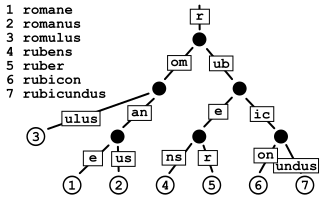
\includegraphics[width=0.45\textwidth]{PatriciaTrie}
 \caption{Пример Radix tree}
\end{wrapfigure}

Radix tree представляет собой сжатое prefix tree. В свою очередь, prefix tree является
структурой данных, которая предоставляет интерфейс ассоциативного массива и позволяет
хранить значения в виде key-value пар.
В этом исследовании в качестве key выбраны строки, причем в отличие от обычный деревьев,
на ребрах radix tree могут храниться как один элемент (символ),
так и последовательность элементов (строка).

Radix tree широко применяется в ядре Linux для связи указателя с длинным целочисленным ключом.
Эта структура данных эффективна с точки зрения скорости поиска и хренения информации.
В то же время, Radix tree применяется в IP-адресации, так как очень удобна для хранения
иерархической структуры IP-адресов.

Рассмотрим подробнее характеристики radix tree. Пусть требуется хранить ключи размером k
при хранении n элементов в дереве. Тогда добавление элемента, поиск и удаление элемента
занимают $O(k)$ операций.

Для многих запросов поиска по словарю radix tree может быть быстрее и эффективнее, чем хеш-таблицы.
Несмотря на то, что обычно сложность поиска по хэш таблице принимают за $O(1)$,
при этом игнорируется необходимость сначала хешировать входные данные.
На это обычно требуется $O(k)$ операций, где k -- длина входной строки.
Radix tree выполняет поиск за $O(k)$, без необходимости сначала хешировать и имеют гораздо лучшую локальность кеша.
Они также сохраняют порядок, позволяя выполнять упорядоченное сканирование,
получать минимальные / максимальные значения, сканировать по общему префиксу и т.д.

Благодаря всем этим преимуществам, radix tree широко распространено в базе данных Redis, программных продуктах
компании HashiCorp, таких как Terraform, Consul, Vault, Nomad и т.д.,
что представляет дополнительный интерес для его изучения на текстовых данных и сравнения с suffix array.

\textbf{Сжатое представление данных}

Одной из главных задач этой работы является разработка сжатого хранения индекса для suffix array.
Поэтому важно определить, какие данные можно считать сжатыми.

Существуют различные степени сжатости информации.
Предположим, что для хранения некоторого количества данных требуется Z бит.
Сжатые (succinct) структуры данных занимают \(Z + o(Z)\) бит, implicit -- \(Z + o(1)\) бит и
compact -- \(O(Z)\)) бит. В этой работе предлагается сжать suffix array, представив его в succinct виде.
Таким образом, размер массива немногих больше превосходит размер исходного текста.

\textbf{$\Psi$-массив}

Важным место в теории сжатого представления индекса занимает промежуточный $\psi$-массив.
Характерной особенностью всех алгоритмов сжатия succinct suffix array (CSA)
является то, что сжимается не непосредственно индекс, а его представление
в виде $\psi$-массива. Вспомогательный массив можно получить из suffix array путем следующих манипуляций с индексами.
\newpage
Рассмотрим построение $\psi$-массива на примере знакомой строки \textbf{mississippi\$}:
\\ \textbf{Text}:\,\,\,\,\,\,\,\,\,\,\,\,\,\,\,\,\,\,\,\,\,\,\,\, m \,i \,\,\,\,s \,\,\,s \,\,\,\,i \,\,\,\,s \,\,\,s \,\,i \,\,p \,\,p \,\,i \,\,\,\,\$
\\ \textbf{Offset}:\,\,\,\,\,\,\,\,\,\,\,\,\,\,\,\,\,\,\,\, 0 \,\,1 \,\,\,\,2 \,\,3 \,\,\,4 \,\,\,5 \,\,6 \,7 \,\,8 \,\,9 \,10 11
\\ \textbf{Suffix Array}:   11 10 \,7 \,\,4 \,\,\,1 \,\,\,0 \,\,9 \,8 \,\,6 \,\,3 \,\,5 \,\,2
\\ \textbf{$\Psi$ -array}: \,\,\,\,\,\,\,\,\,\,\,\,\$ \,\,\,0 \,\,\,\,7 10 \,\,11 4 \,\,1 \,6 \,\,2 \,\,3 \,\,8 \,\,9

Будем называть потомком (successor) самый большой суффикс подстроки, кроме исходной подстроки.
Т.е. для подстроки issippi\$ потомком является ssippi\$.
$\Psi$-массив указывает на потомок для каждого выбранного суффикса.
Например, рассмотрим $SA[7] = 8$. Его потомком является позиция в suffix array, которая хранит $8 + 1 = 9$.
Таким образом, $\psi[7] = 6$. Главное соотношение между $\Psi$-массивом и suffix array:
\[SA[i] = SA[\psi[i]] - 1\]
Необходимо отметить, что $\Psi[0] = \$$, т.к. для первого элемента в suffix array нет потомка.
При этом $SA[5]$ ссылается на 0-й индекс, то есть на всю строку целиком.
Иными словами, элемент suffix array ссылается на начало текста,
т.е. никакой другой суффикс не может иметь его в качестве потомка.
Соответственно в $\psi$-массиве нет элемента, равного 5.

\textbf{Восстановление suffix array из $\psi$-массива}

Существует возможность восстановить исходный suffix array по сгенерированному $\psi$-массиву
фактически с помощью операций, обратных к тем, которые были представлены в предыдущем параграфе.
Коснемся подробнее особенностей работы этого алгоритма.

В первую очередь необходимо найти индекс элемента suffix array, который не встречается в $\psi$-массиве.
В нашем примере он равен 5. Из приведенных выше рассуждений следует, что $SA[5] = 0$.
Таким образом был декодирован один элемент исходного suffix array. Из формулы ... для $i = 5$ следует:

\[SA[5] = SA[\psi[5]] - 1\]
\[0 = SA[4] - 1\]
\[SA[4] = 1\]

Еще один элемент suffix array восстановлен! Таким образом можно восстановить всю оставшуюся последовательность.
Время на поиск первого элемента составляет \(O(n)\) операций.
Существуют некоторые улушения скорости поиска нужного элемента в suffix array, требующие дополнительных
структур данных, хранящих значение suffix array на каждом \(\log n\) шаге. Такой способ выходит за рамки этой работы,
поскольку главной задачей является максимальное сжатие индекса.

\textbf{Сжатие $\psi$-массива}

Рассмотрим подробнее $\psi$-массив:
\\ \textbf{Text}:\,\,\,\,\,\,\,\,\,\,\,\,\,\,\,\,\,\,\,\,\,\,\,\, m \,i \,\,\,\,s \,\,\,s \,\,\,\,i \,\,\,\,s \,\,\,s \,\,i \,\,p \,\,p \,\,i \,\,\,\,\$
\\ \textbf{Offset}:\,\,\,\,\,\,\,\,\,\,\,\,\,\,\,\,\,\,\,\, 0 \,\,1 \,\,\,\,2 \,\,3 \,\,\,4 \,\,\,5 \,\,6 \,7 \,\,8 \,\,9 \,10 11
\\ \textbf{Suffix Array}:   11 10 \,7 \,\,4 \,\,\,1 \,\,\,0 \,\,9 \,8 \,\,6 \,\,3 \,\,5 \,\,2
\\ \textbf{$\Psi$ -array}: \,\,\,\,\,\,\,\,\,\,\,\,\$ \,\,\,0 \,\,\,\,7 10 \,\,11 4 \,\,1 \,6 \,\,2 \,\,3 \,\,8 \,\,9

Отсортированный набор суффиксов имеет вид:
\\ (0) \,\,\,\$
\\ (1) \,\,\,i\$
\\ (2) \,\,\,ippi\$
\\ (3) \,\,\,issippi\$
\\ (4) \,\,\,ississippi\$
\\ (5) \,\,\,mississippi\$
\\ (6) \,\,\,pi\$
\\ (7) \,\,\,ppi\$
\\ (8) \,\,\,sippi\$
\\ (9) \,\,\,sissippi\$
\\ (10) ssippi\$
\\ (11) ssissippi\$

Стоит обратить внимание на его структуру: он состоит из набора возрастающих последовательностей индексов.
Рассмотрим возрастающую последовательность 2, 3, 8, 9.

$SA[2] = 7$, $T[7] = i$.
$SA[3] = 4$, $T[4] = i$. Примечательно, что $SA[6] = 9$, $T[9] = p$.
То есть чередование индексов с возрастания на убывание соответствует смене символа с i на p.

\begin{theorem}
 \label{lemma:1}
 Два последовательных элемента $\psi$-массива являются возрастающими, если соответствующие суффиксы,
 на которые они ссылаются, начинаются с одного и того же символа.
\end{theorem}

\begin{proof}
 По построению, suffix array представляет собой набор индексов в исходном тексте,
 отсортированный в лексикографическом порядке. Это означает, что $T[SA[i]] < T[SA[i + 1]]$
 $\forall i \in [0, n).$ Эти два суффикса имеют общий первый символ. Поэтому они отличаются в следующих
 элементах, например, во втором: $T[SA[i] + 1] < T[SA[i + 1] + 1].$

 $\Psi$-массив ссылается на потомка для данного суффикса: $T[SA[\psi[i]]] < T[SA[i] + 1].$
 Т.к. $T[SA[i]]$ и $T[SA[i + 1]]$ имеют одинаковый первый символ, их потомки упорядочены.
 Если $T[SA[\psi[i]]] < T[SA[\psi[i + 1]]]$, тогда из-за упорядоченности индекс в suffix array
 для первого должен находиться перед индексом для второго. Следовательно индексы (значения $\psi$-массива)
 должны быть упорядочены, если суффиксы имеют общий первый символ.
\end{proof}

Возрастающие последовательности неотрицательных целых чисел сжимаемы.
Самый простой путь для хранения таких последовательностей -- битмап.
Однако этот способ не позволяет иметь произвольный доступ к элементам.
Рассмотрим более совершенный алгоритм сжатого представления данных.

\textbf{Кодировка Elias--Fano}

Сжатие при помощи метода Elias--Fano позволяет представлять монотонно возрастающие последовательности
целых неотрицательных чисел в виде битовых векторов. Этот способ делает возможным
хранение неубывающей последовательности $n$ целых чисел размером $[0, m)$,
занимая $2n + n[\log m/n]$ бит, предоставляя доступ к $i$-му элементу за $O(1)$.
Сравнив размеры структуры данных с минимально возможным занимаемым местом в памяти
с точки зрения теории информации, Elias--Fano кодировка является сжатым (succinct) индексом.

\begin{figure}[t]
 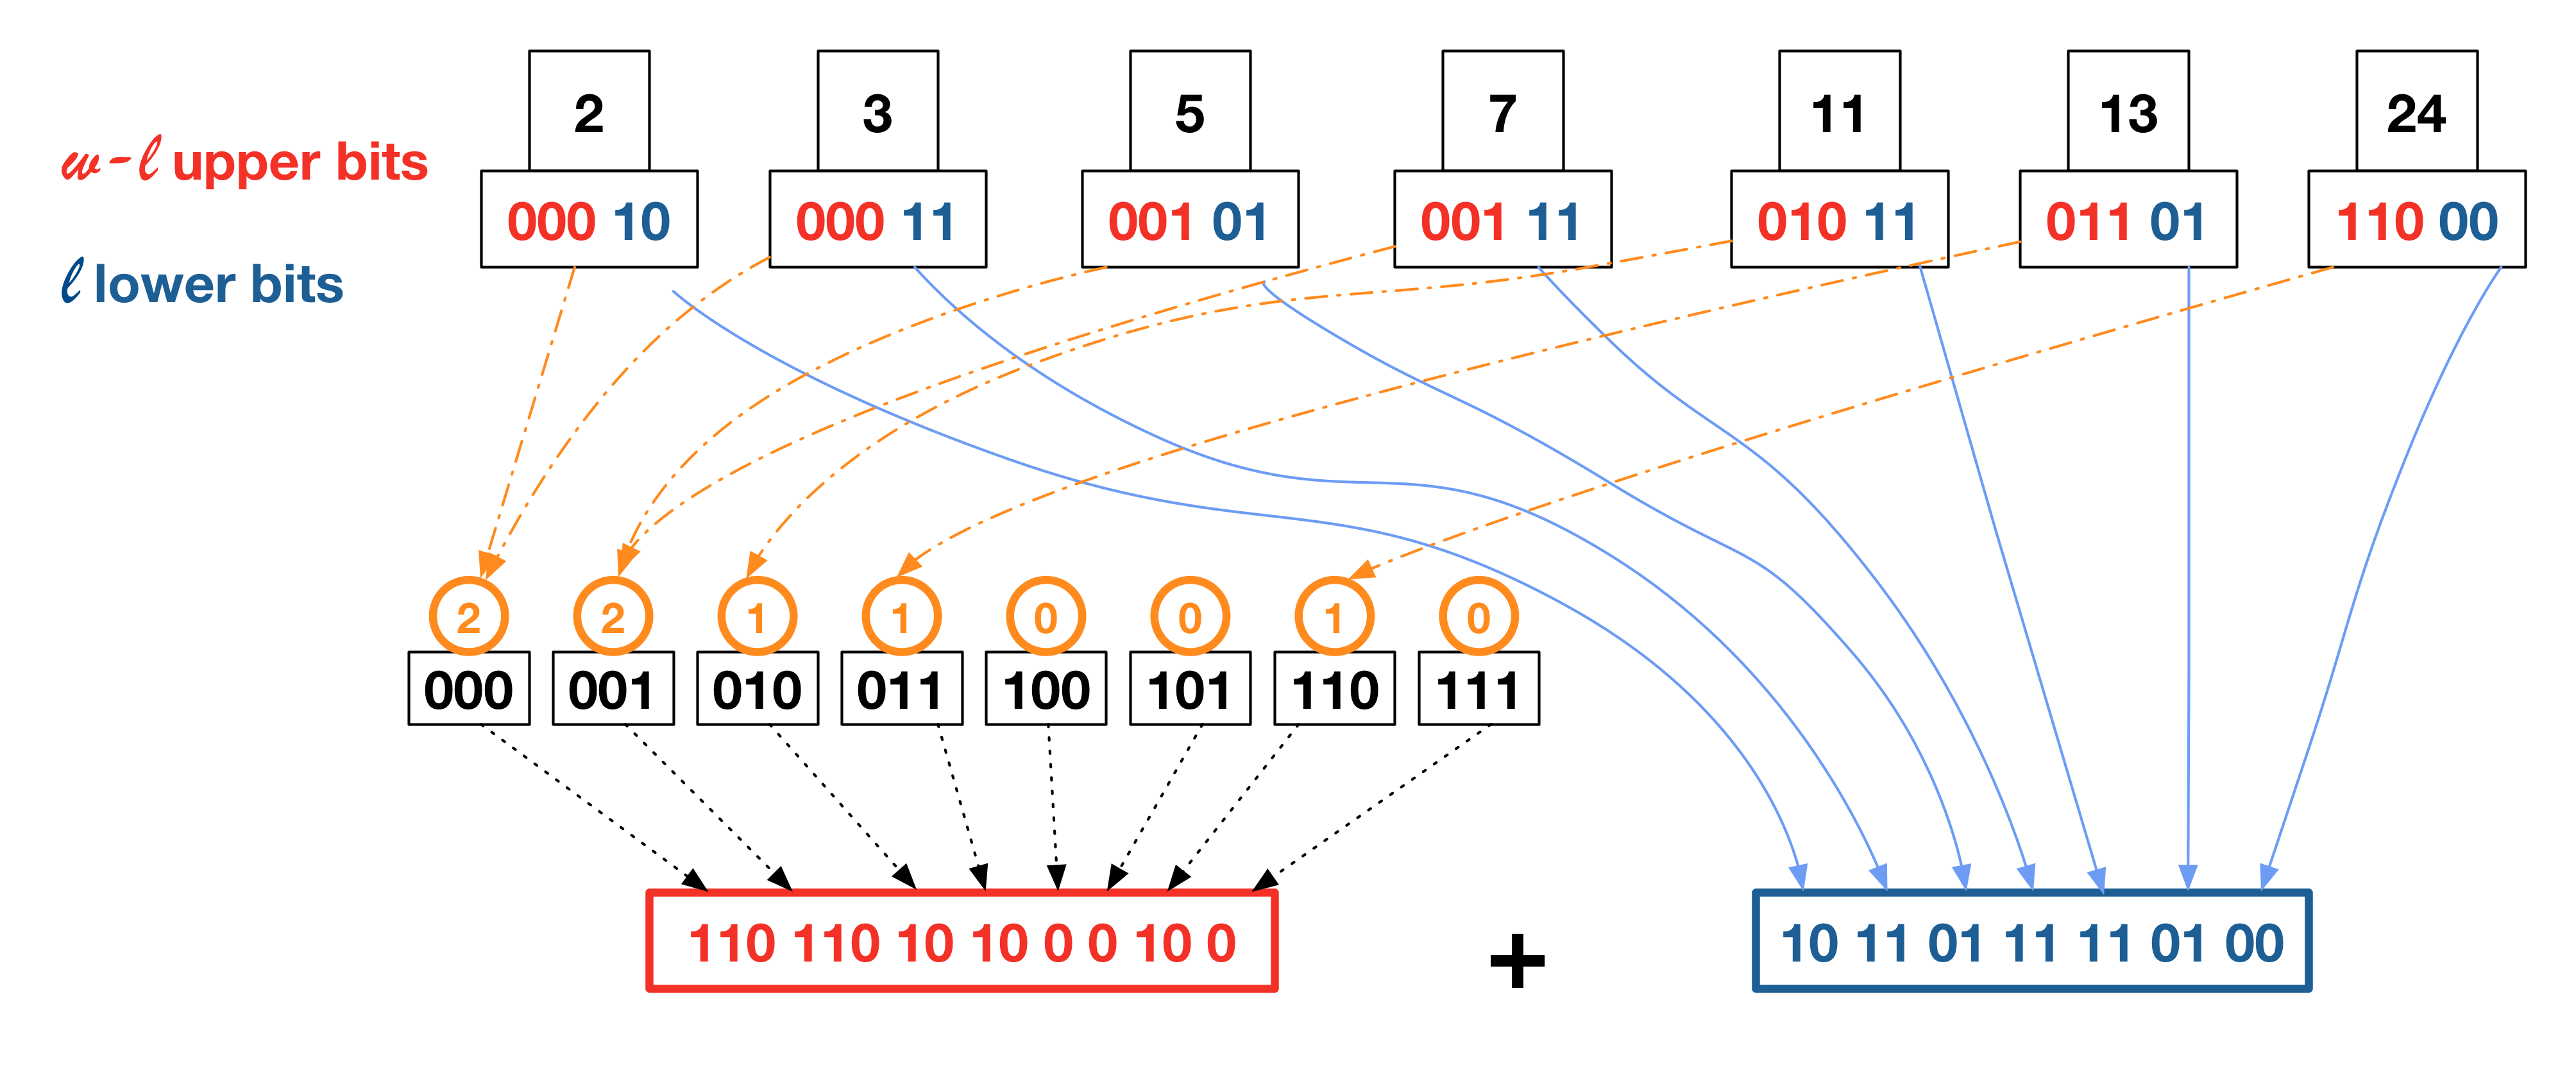
\includegraphics[width=12cm]{Elias-Fano}
 \caption{Пример построения кода Elias-Fano}
 \centering
 \label{fig:EF}
\end{figure}

В начале каждое число из последовательности кодируется $\log m$ битами данных.
Двоичное представление элементов разбито на две части: верхнюю часть, содержащую в себе
первые $\log n$ бит, и нижнюю, с оставшимися $\log m - \log n = \log m / n$ бит.
Объединение нижних битов занимает $n \log m$ бит. Верхние биты представляют собой
набор из $n + m / 2^{\log m/n}$ бит. Начиная с пустого битового вектора, мы добавляем в эту часть 0
в качестве стоп-бита для каждого возможного значения, представляемого битами старшей части.
Мы добавляем 1 для каждого фактически присутствующего значения, выставляя его перед соответствующим стоп-битом.

В качестве примера рассмотрим отсортированную последовательность {2,3,5,7,11,13,24}.
На рисунке \ref{fig:EF} показана схема кодирования. Наибольшим числом в наборе (universe) является 24.
Поэтому для представления каждого элемента необходимо выделить 5 бит на элемент.
Затем нужно разбить бинарное представление на две части: верхнюю и нижнюю.
Исходя из ранее оговоренных условий, выберем 3 бита под верхнюю часть и 2 бита под нижнюю.
Всего в последовательности присуствует 7 элементов. Рассмотрим число 2. Для него имеем
$2 = 0b00010$ и соответственно 000 в качестве верхней части и 10 в качестве нижней.
Повторяя этот процесс, получим набор нижних частей для каждого элемента.
Затем объединим полученные чати вместе. Для верхних частей имеется $2^3$ вариантов
наборов значений. С каждым таким набором асссоциируется счетчик, который увеличивается на единицу,
если число из последовательности имеет соответствующую верхнюю часть.
Так для 2 инкрементируем набор 000. Число $3 = 0b00011$ с верхней частью 000 идет в тот же набор.
Для числа $5 = 0b00101$ с верхней частью 001 инкрементируем набор 001 и т.д.
Наконец, кодируем счетчики унарно, добавляя столько единиц в представление счетчика,
сколько имеет значение каждого счетчика, за которым следует 0 бит.
Окончательное кодирование Elias-Fano получается объединением полученных верхней и нижней частей.

\textbf{Восстановление данных из кода Elias--Fano}

Для восстановления исходной монотонной нецбывающей последовательности чисел, необходимо разработать операцию
доступа к $i$-му элементу последовательности, $i \in [0, n)$. Для доступа к нижней части
достаточно просто получить соответствующие биты, т.к. длина вектора для хранения элемента известна.
Для получения старшей части, необходимо осуществить операцию \emph{select}.
Операция \emph{select($i$)} позволяет получить позицию $i$-го бита, выставленного в 1 в битовом векторе.
Эта операция может быть выполнена за $O(1)$, что позволяет получать произвольный доступ к элементу
последовательности без полного раскодирования всей последовательности целиком.

\newpage
\section{Исследование}
% Add texts overview.
% table of texts

Исследование состоит из нескольких главных частей. В первую очередь реализуется изучение работы традиционной структуры
данных suffix array с точки зрения потребляемой памяти, времени построения индекса и поиска подстроки.
Затем исследуется более современное radix tree, в котором обозреваются аналогичные аспекты функционирования.
Одной из важнейших частей работы является разработка сжатого суффиксного массива (CSA).
При этом выполняется не только тестирование CSA на бенчмарках, подобных другим обозреваемым структурам данных,
но и исследование степени сжатия индекса по сравнению с suffix array.
Важно подчеркнуть, что особый интерес представляет сравнение работы алгоритмов на текстах разного содержания.

\newpage
\subsection{Экспериментальная платформа}
Исследование, включающее в себя запуск бенчмарков, велось на машине с характеристиками,
указанными в таблице \ref{table:1}.
\begin{table}[h!]
    \centering
    \begin{tabular}{|c|c|}
        \hline
        CPU & Intel Core i5-9600K 3.70 GHz\\
        \hline
        RAM & 16GB \\
        \hline
        System Type & 64-bit\\
        \hline
        Operating System & Windows 10\\
        \hline
        L1 Cache & 512 B\\
        \hline
        L2 Cache & 1 KB\\
        \hline
        L1 Cache & 10 KB\\
        \hline
    \end{tabular}
    \caption{Характеристики компьютера}
    \label{table:1}
\end{table}

\newpage
\subsection{Suffix array}
% overview +
% complexity +
% code snippet +
% measurements +
% table +

Для анализа работы структуры данных взят suffix array из стандартной библиотеки языка Go.
% https://golang.org/pkg/index/suffixarray/
Он принимает на вход текст и составляет из него отсортированный индекс, с помощью которого можно осуществлять
операции поиска подстроки. Создание индекса занимает $O(n)$ операций, где $n$ -- размер исходного текста.
Поиск подстроки занимает $O(\log n \cdot |s|)$, где $|s|$ -- это длина искомой подстроки.
Рассмотрим подробнее бенчмарки. Исходный текст загружается из файла, затем выбирается подстрока,
ограниченная позициями $[leftPos:rigtPos]$.

\begin{lstlisting}[caption=Suffix array example]
func BenchmarkLookup(b *testing.B, testStr []byte) {
    sa := suffixarray.New(testStr)
    b.ResetTimer()
    for i := 0; i < b.N; i++ {
        offset := sa.Lookup(testStr[leftPos: rightPos], -1)
        if len(offset) < 1 || offset[0] != leftPos {
            b.Fatalf("mis-match: %v", offset)
        }
    }
}
\end{lstlisting}

На листинге 1 показан упрощенный код бенчмарка поиска подстроки для suffix array
(маловажные для общего понимания детали опущены). Код протестирован для 5 текстов разного содержания.
Размер подстроки для поиска данных является одинаковым для каждого измерения.

\begin{table}[h!]
    \centering
    \begin{tabular}{|c|c|c|}
        \hline
        Размер текста, KB & Память, KB & Время, s\\
        \hline
        9766 & 58741 & 1.832\\
        \hline
        977 & 6020 & 0.337\\
        \hline
        879 & 5457 & 0.333\\
        \hline
        782 & 4838 & 0.323\\
        \hline
        684 & 4252 & 0.314\\
        \hline
        586 & 3669 & 0.305\\
        \hline
        489 & 3589 & 0.297\\
        \hline
        391 & 2925 & 0.285\\
        \hline
        293 & 2244 & 0.275\\
        \hline
        196 & 1563 & 0.274\\
        \hline
        98 & 881 & 0.260\\
        \hline
        49 & 547 & 0.258\\
        \hline
        10 & 246 & 0.252\\
        \hline
        5 & 212 & 0.251\\
        \hline
        2 & 194 & 0.256\\
        \hline
    \end{tabular}
    \caption{Построение suffix array}
    \label{table:2}
\end{table}

Т.к. размер suffix array не зависит от размера алфавита,
результаты для разных текстов отличаются в пределах погрешности измерения,
поэтому для наглядности достаточно привести пример для одного типа текста.
В таблице \ref{table:2} показаны результаты измерений построения индекса для Amazon Text Corpora.

% size, kb: 977, 879, 782, 684, 586, 489, 391, 293, 196, 98
% time, mks: 12251, 11857, 12331, 12969, 12777, 12680, 11795, 11555, 11752, 11657
% mem, kb:  6101, 5501, 4915, 4333, 3747, 3707, 3001, 2322, 1642, 962

\begin{table}[h!]
    \centering
    \begin{tabular}{|c|c|c|}
        \hline
        Размер текста, KB & Память, KB & Время, ms\\
        \hline
        977 & 6020 & 12.251\\
        \hline
        879 & 5457 & 11.857\\
        \hline
        782 & 4838 & 12.331\\
        \hline
        684 & 4252 & 12.969\\
        \hline
        586 & 3669 & 12.777\\
        \hline
        489 & 3589 & 12.680\\
        \hline
        391 & 2925 & 11.795\\
        \hline
        293 & 2244 & 11.555\\
        \hline
        196 & 1563 & 11.752\\
        \hline
        98 & 881 & 11.657\\
        \hline
    \end{tabular}
    \caption{Поиск подстроки в suffix array}
    \label{table:3}
\end{table}


\newpage
\subsection{Radix tree}
Реализация radix tree на языке Go взята из следующего источника: \cite{golang2016sa}
Во многом выбор обусловлен удобством встраивания бенчмарка в существующую систему тестирования на языке Go.
При этом с алгоритмической точки зрения эта реализация подтверждает
теоретическое описание сложности поиска подстроки за $O(1)$.
\newpage
\begin{lstlisting}[caption=Radix tree example]
func BenchmarkConstruct(b *testing.B, testStr string) {
	var substringArray []string = createSubstrings(testStr)
	b.ResetTimer()
	r := radix.New()
	for i := 0; i < b.n; i++ {
		fillRadixTree(b.N, r, substringArray)
	}
}
\end{lstlisting}

На приведенном листинге 2 в кратком виде показана функция построения radix tree.
В начале генерируется набор подстрок из текста, прочитанного из файла. В функции $fillRadixTree$
происходит добавление подстрок в дерево. Сравнительные характеристики построения radix tree
для Amazon Text Corpora \cite{amazon2013text} приведены в таблице \ref{table:4}.

% size, kB: 196, 148, 98, 79, 49, 10, 5, 2
% time, s:  276.419, 128.494, 57.319, 36.786, 14.632, 0.845, 0.414, 0.284
% mem, KB:  20248160, 11501051, 5192071, 3353864, 1324283, 52803, 13528, 2314

\begin{table}[h!]
    \centering
    \begin{tabular}{|c|c|c|}
        \hline
        Размер текста, KB & Память, MB & Время, s\\
        \hline
        196 & 20248 & 276.419\\
        \hline
        148 & 11501 & 128.494\\
        \hline
        98 & 5192 & 57.319\\
        \hline
        79 & 3353 & 36.786\\
        \hline
        49 & 1324 & 14.632\\
        \hline
        10 & 52 & 0.845\\
        \hline
        5 & 13 & 0.414\\
        \hline
        2 & 2 & 0.284\\
        \hline
    \end{tabular}
    \caption{Построение radix tree}
    \label{table:4}
\end{table}

Ниже в листинге 3 приведен упрощенный пример функции поиска подстроки в дереве.
Построенная структура показывает очень хороший результат поиска подстроки за константное время.
Его можно видеть в таблице \ref{table:5}.

\newpage
\begin{lstlisting}[caption=Radix tree lookup]
func getSubstring(r *radix.Tree,
                  subString string, testStr string) {
	var out interface{}
	var pos interface{}
	// there is only one possible match for a string
	fn := func(s string, v interface{}) bool {
		out, pos = s, v
		return false
	}
	r.WalkPrefix(subString, fn)
	return out.(string), pos
}
\end{lstlisting}

% size, kB: 20, 50, 60, 70, 80, 90, 100, 120, 150
% time, ns: 220, 242, 243, 237, 243, 244, 243, 245, 256
% mem, KB:  212243, 1334534, 1918371, 2595544, 3370035, 4237366, 5210522, 7449706, 11529887

\begin{table}[h!]
    \centering
    \begin{tabular}{|c|c|c|}
        \hline
        Размер текста, KB & Память, MB & Время, s\\
        \hline
        150 & 11529 & 256\\
        \hline
        120 & 7449 & 245\\
        \hline
        100 & 5210 & 243\\
        \hline
        90 & 4237 & 244\\
        \hline
        80 & 3370 & 243\\
        \hline
        70 & 2595 & 237\\
        \hline
        60 & 1918 & 243\\
        \hline
        50 & 1334 & 242\\
        \hline
        20 & 212 & 220\\
        \hline
    \end{tabular}
    \caption{Поиск подстроки в radix tree}
    \label{table:5}
\end{table}


\newpage
\subsection{Compressed suffix array}
% structure +
% create index +
% create psi +
% bitmap +
% auxiliary data structures +
% ef +
% decode bv->psi +
% decode psi->sa +
% final structure +
% search sa
% complexity +

Перейдем к описанию реализации CSA. Как было упомянуто в обзоре литературы, для начала необходимо
построить индекс таким же способом, как это происходит в suffix array.
Для этого требуется $O(n)$ операций \cite{huo2014practical}.

\textbf{Структура CSA}

\begin{lstlisting}[caption=CSA structure]
type Csa struct {
	text            string
	suffixOffsets   []int
	psi             []uint64
	length          int
}
\end{lstlisting}

На приведенном выше листинге 4 обозначена упрощенная структура CSA. Она состоит из исходного текста
(сжимается только индекс, текст остается в прежнем виде), индекса, $\psi$-массива и длины текста.
Индекс строится с помощью функции, в которой за основу алгоритма взят алгоритм построения suffix array
из библиотеки языка Go \cite{golang2016sa}.

\textbf{Построение $\psi$-массива}

Для построения $\psi$-массива нужно принять $\psi[0] = \$$. Затем произвести итеративный обход
suffix array и найти индекс, соответствующее значение которого в suffix array совпадает с текущим,
увеличенным на единицу. В листинге 5 показан псевдокод алгоритма.

\begin{lstlisting}[caption=Построение CSA]
func ConstructPsi() {
	for i < len {
		if sa[j] = sa[i] + 1 {
			psi[i] = j
		}
	}
}
\end{lstlisting}

\textbf{Вспомогательные структуры данных}

Для хранения данных используется битмап (bitmap) из пакета\\ Roaring.bitmap \cite{chambi2016better}.
Это быстрая и эффективная реализация битмапа. Также Roaring используется во многих продуктах,
таких как Apache Druid, LinkedIn Pinot, Google Procella и т.д.

Полученный $\psi$-массив представляет собой набор монотонно неубывающих последовательностей чисел.
Алгоритм Elias-Fano позволяет преобразовывать каждую такую последовательность в битвектор в отдельности.
Количество этих последовательностей совпадает с размером алфавита, используемого в тексте \cite{andersensimple}.
Возникает вопрос, каким образом можно организовать хранение таких битвекторов.

Одним из решений является использование двух дополнительных массивов:
первый для хранения оступа в $\psi$-массиве, второй для хранения символа,
соответствующего возрастающей последовательности.
В этой работе кодировка текста представляет собой ASCII-код или код меньшего размера.
Таким образом, размер алфавита ограничен 128 символами. Следовательно, размер
дополнительных массивов не превышает $2 \cdot m$, где $m$ -- размер алфавита.
Массив с оступами используется для быстрого индексирования по массиву битмапов.

Заполнение дополнительных структур данных и расчет отступов происходит при сжатии каждой отдельной
монотонной неубывающей последовательности индексов.
Для отделения таких последовательностей используется описанное ранее свойство из Леммы \ref{lemma:1}.
Нарушение возрастания $\psi$-массива соответсвует смене символа. Таким образом можно идексировать
битмапы и заполнить вспомогательный массив с символами используемого алфавита.

\textbf{Elias-Fano}

Сжатие при помощи алгоритма Elias-Fano осуществляется для каждой отдельной последовательности.
При этом происходит предварительное построение верхней и нижней частей (младших и старших биты)
битового представления чисел из этой последовательности. Рассчитывается отступ для дальнейшего
быстрого доступа к младшим битам. В процессе сжатия числа записываются в битмап,
в котором можно индексироваться за константное время.

Для того чтобы получить доступ к элементу последовательности (части $\psi$-массива),
необходимо использовать функцию $select(i)$, реализованную в битмапе, работающую за $O(1)$.
Для проверки корректности работы алгоритма реализована функция получения всего $\psi$-массива
при помощи вызова $select(i)$.

\textbf{Восстановление suffix array}

Для получения доступа к элементу suffix array $sa[i]$ нет необходимости полностью декодировать
$\psi$-массив. Для этого требуется осуществить проход по $\psi$-массиву, пока не будет достигнут
последний элемент. Сосчитав количество шагов до последнего элемента $h(i)$, найдем индекс искомого
значения путем несложного вычисления: $sa[i] = n - h(i)$. Такой алгоритм требует $O(n)$ операций \cite{andersensimple}.

\textbf{Окончательная структура CSA}

После добавления вспомогательных данных структура CSA принимает вид, показанный на листинге 6

\newpage
\begin{lstlisting}[caption=CSA structure]
type Csa struct {
	text      string
	bv        []*CompressedText
	seqOffset []int
	seqChar   []byte
	length    int
	alphLen   int
}
\end{lstlisting}

Важно подчеркнуть, что теперь нет необходимости хранить индексы и вспомогательный $\psi$-массив.
Вместо этого данные хранятся в сжатом виде в последовательности битвекторов.
Кроме того, исходный текст все так же остается в первоначальном виде.

Таким образом, для хранения сжатого индекса требуется $n \cdot \log |\sigma| + o(n)$,
где $|\sigma|$ -- размер алфавита. При двоичном поиске по suffix array необходимо произвести $O(\log n)$ операций.
Для получения индекса в suffix array из $\psi$-массива требуется осуществить $O(n)$ операций.
Суммарно для поиска элемента требуется $O(n\cdot \log n)$ операций.

\textbf{Тестирование CSA}

Рассмотрим эффективность работы CSA на примере пяти текстов различного содержания.
Для начала оценим время построения массива и требуемое количество памяти для его хранения.
В таблице \ref{table:6} указаны данные для Amazon Text Corpora.

% csa_len = [879, 782, 684, 586, 498, 391, 293, 196, 98, 49, 10, 5, 2] # amazon
% csa_time = [392.040, 299.721, 225.818, 165.427, 114.660, 73.818, 41.825, 18.803, 4.981, 1.431, 0.313, 0.269, 0.256] # amazon
% csa_mem = [2281, 2036, 1816, 1573, 1336, 1082, 817, 561, 309, 163, 45, 26, 17] # amazon

\begin{table}[h!]
	\centering
	\begin{tabular}{|c|c|c|}
		\hline
		\multicolumn{3}{|c|}{Amazon} \\
		\hline
		Размер текста, KB & Память, MB & Время, s\\
		\hline
		879 & 2281 & 392.040\\
		\hline
		782 & 2036 & 299.721\\
		\hline
		684 & 1816 & 225.818\\
		\hline
		586 & 1573 & 165.427\\
		\hline
		489 & 1336 & 114.660\\
		\hline
		391 & 1082 & 73.818\\
		\hline
		293 & 817 & 41.825\\
		\hline
		196 & 561 & 18.803\\
		\hline
		98 & 309 & 4.981\\
		\hline
		49 & 163 & 1.431\\
		\hline
		10 & 45 & 0.313\\
		\hline
		5 & 26 & 0.269\\
		\hline
		2 & 17 & 0.256\\
		\hline
	\end{tabular}
	\caption{Построение CSA}
	\label{table:6}
\end{table}

% csa_len = [977, 879, 782, 684, 586, 489, 391, 293, 196, 98, 49, 10, 5, 2] # dna
% csa_time = [491.614, 385.973, 309.387, 232.106, 168.735, 116.836, 73.656, 42.861, 18.788, 4.922, 1.446, 0.304, 0.267, 0.255] # dna

%\begin{table}[h!]
%	\centering
%	\begin{tabular}{|c|c|c|}
%		\hline
%		\multicolumn{3}{|c|}{DNA} \\
%		\hline
%		Размер текста, KB & Память, MB & Время, s\\
%		\hline
%		977 & 2011 & 491.614\\
%		\hline
%		879 & 1782 & 285.973\\
%		\hline
%		782 & 1547 & 309.387\\
%		\hline
%		684 & 1396 & 232.106\\
%		\hline
%		586 & 1228 & 168.735\\
%		\hline
%		489 & 1077 & 116.836\\
%		\hline
%		391 & 845 & 73.656\\
%		\hline
%		293 & 627 & 42.861\\
%		\hline
%		196 & 436 & 18.788\\
%		\hline
%		98 & 241 & 4.922\\
%		\hline
%		49 & 124 & 1.446\\
%		\hline
%		10 & 34 & 0.304\\
%		\hline
%		5 & 23 & 0.267\\
%		\hline
%		2 & 16 & 0.255\\
%		\hline
%	\end{tabular}
%	\caption{Построение CSA}
%	\label{table:7}
%\end{table}

\begin{figure}[h!]
	\centering
	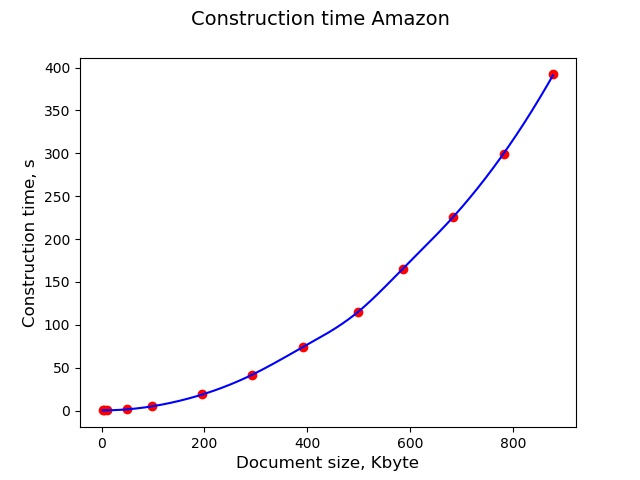
\includegraphics[width=12cm]{construct_time_amazon}
	\caption{Построение CSA}
	\label{fig:CSA_construct_time_amazon}
\end{figure}

\begin{figure}[h!]
	\centering
	\begin{subfigure}[b]{0.49\textwidth}
		\centering
		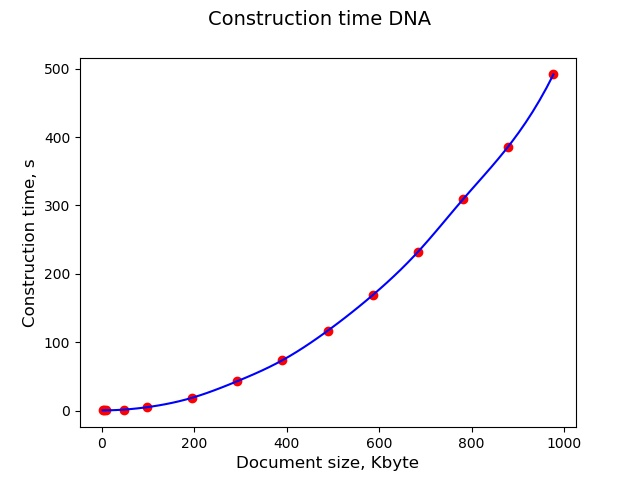
\includegraphics[width=\textwidth]{construct_time_DNA}
		\caption{DNA}
		\label{fig:y equals x}
	\end{subfigure}
	\hfill
	\begin{subfigure}[b]{0.49\textwidth}
		\centering
		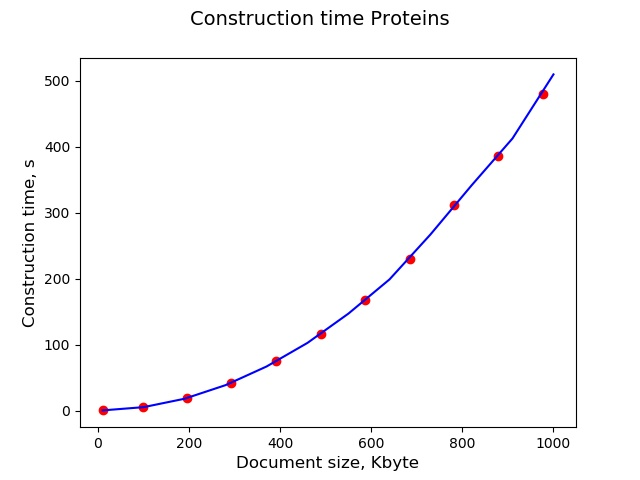
\includegraphics[width=\textwidth]{construct_time_Proteins}
		\caption{Proteins}
		\label{fig:three sin x}
	\end{subfigure}
	\hfill
	\begin{subfigure}[b]{0.49\textwidth}
		\centering
		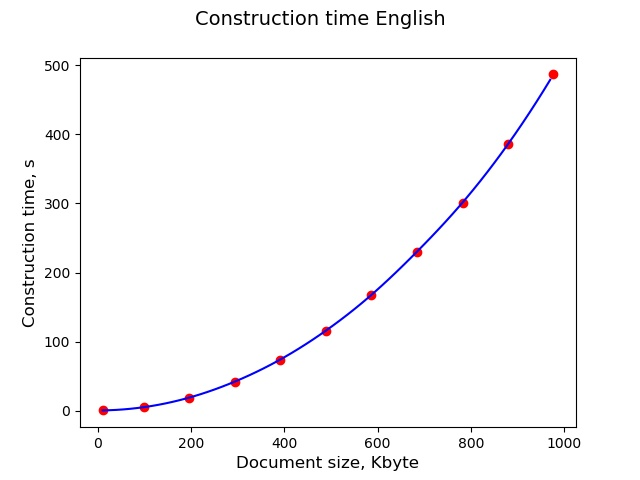
\includegraphics[width=\textwidth]{construct_time_English}
		\caption{English}
		\label{fig:three sin x}
	\end{subfigure}
	\hfill
	\begin{subfigure}[b]{0.49\textwidth}
		\centering
		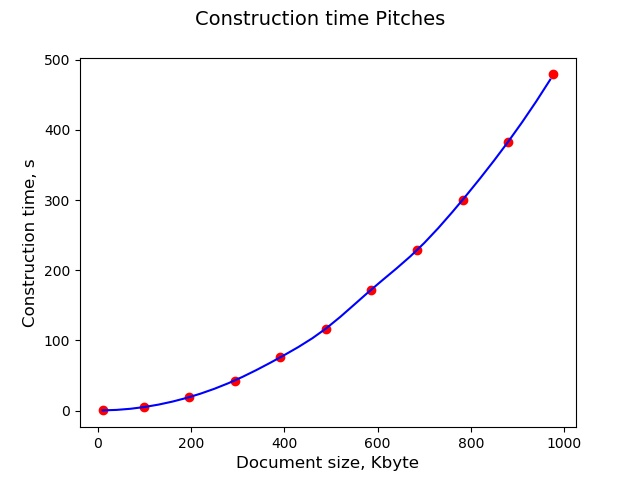
\includegraphics[width=\textwidth]{construct_time_Pitches}
		\caption{Pitches}
		\label{fig:three sin x}
	\end{subfigure}
	\caption{Построение CSA}
	\label{fig:three graphs}
\end{figure}

\begin{figure}[h!]
	\centering
	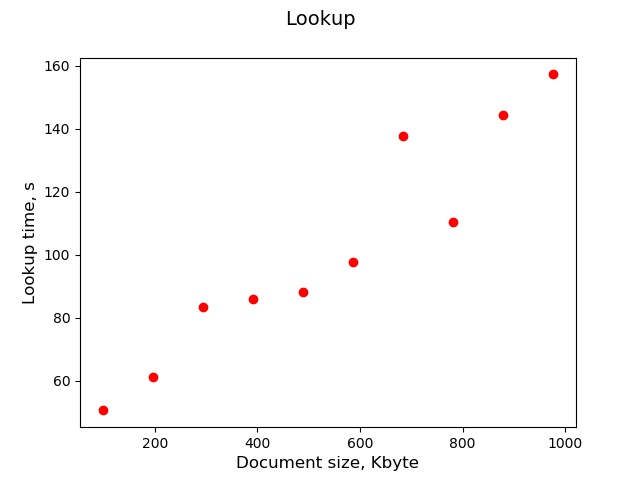
\includegraphics[width=12cm]{Lookup_time_csa_amazon}
	\caption{Поиск подстроки в CSA}
	\label{fig:CSA_Lookup_time_csa_amazon}
\end{figure}

\clearpage
\newpage
Рассмотрим результаты зависимость скорости поиска подстроки от размера текста для CSA,
suffix array и radix tree, построенных для Amazon Text Corpora. На рисунке \ref{fig:CSA_Lookup_time}
можно видеть, что скорость поиска подстроки фиксированного размера не зависит от размера текста
для suffix array и radix tree. Для CSA время поиска увеличивается при увеличении размера исходного текста.
Radix tree, как ожидалось, показывает лучший результат.

\begin{figure}[h!]
	\centering
	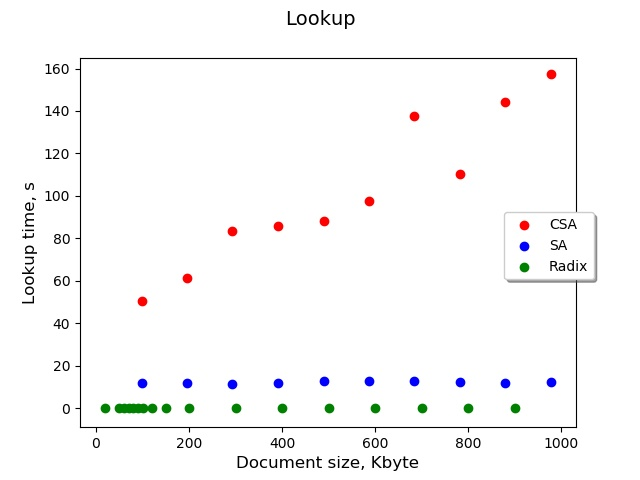
\includegraphics[width=12cm]{Lookup_time}
	\caption{Поиск подстроки в CSA}
	\label{fig:CSA_Lookup_time}
\end{figure}



\newpage
\subsection{Сравнительные измерения}
На рисунке \ref{fig:CSA_Lookup_diff_texts} представлены сравнительные характеристики поиска
подстроки для различных текстовых данных.

\begin{figure}[h!]
    \centering
    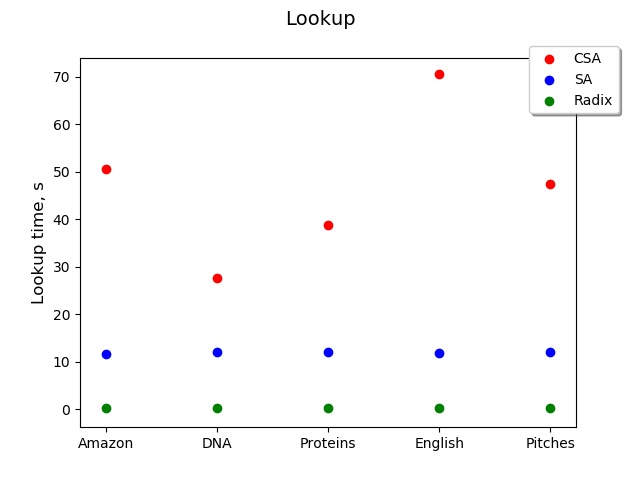
\includegraphics[width=12cm]{lookup_diff_texts}
    \caption{Поиск подстроки в CSA}
    \label{fig:CSA_Lookup_diff_texts}
\end{figure}

Рассмотрим относительное сжатие CSA по сравнению с suffix array. Расчитывается среднее отношение памяти,
затраченной для работы CSA, к памяти, затраченной suffix array в зависимости от длины исходного текста.
На рисунке \ref{fig:CSA_compression_ratio_amazon} можно заметить уменьшение отношения, т.е. увеличение
коэффициента сжатия. Примечательно, что для малых размеров исходного текста CSA занимает больше места,
чем suffix array. Это объясняется наличием дополнительных структур данных, описанных на предыдущих страницах.
При построении CSA они занимают место, сопоставимое по порядку с размером индекса в сжатом виде.
Для больших текстов CSA становится более эффективным по сравнению с классическим suffix array.

\begin{figure}[h!]
    \centering
    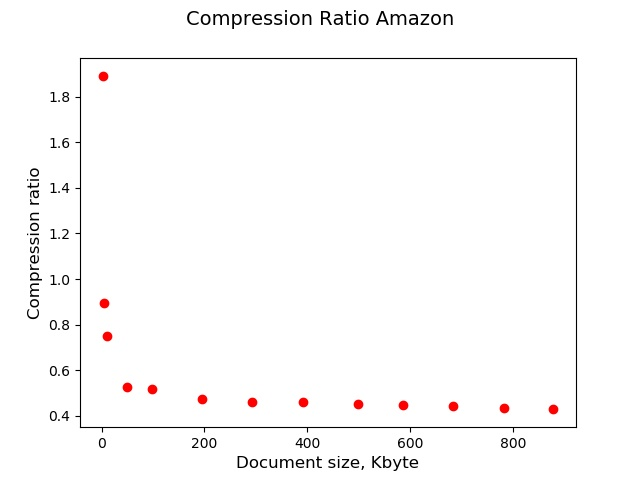
\includegraphics[width=12cm]{compression_ratio_amazon}
    \caption{Сжатие CSA по сравнению с SA}
    \label{fig:CSA_compression_ratio_amazon}
\end{figure}

\clearpage
Относительное сжатие CSA/SA для различных текстов показано на рисунке \ref{fig:CSA_compression_ratio_dif_texts}.
Можно явным образом заметить зависимость размера сжатого индекса от мощности алфавита, чего нельзя
сказать о suffix array и radix tree.

\begin{figure}[h!]
    \centering
    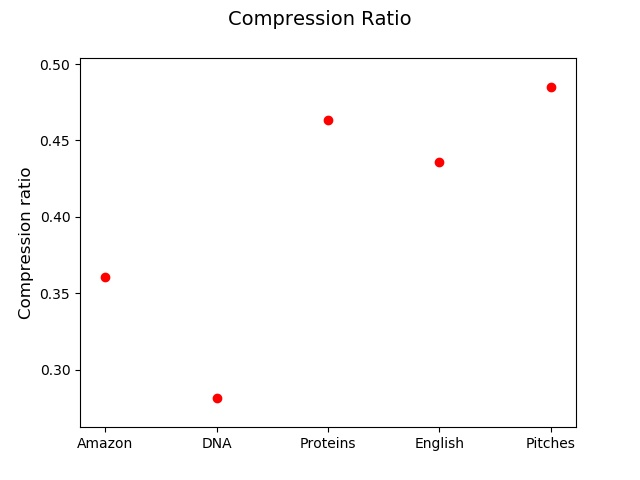
\includegraphics[width=12cm]{compression_ratio_dif_texts}
    \caption{Сжатие CSA по сравнению с SA}
    \label{fig:CSA_compression_ratio_dif_texts}
\end{figure}

\newpage
\section{Выводы}

% insert the text
\newpage
\section{Заключение}

\newpage
\appendix
\section{\\Листинги на языке go}


\end{document}
